%% 美赛模板:正文部分

\documentclass[12pt]{article}  % 官方要求字号不小于 12 号,此处选择 12 号字体

% 本模板不需要填写年份,以当前电脑时间自动生成
% 请在以下的方括号中填写队伍控制号
\usepackage[1234567]{easymcm}  % 载入 EasyMCM 模板文件
\problem{F}  % 请在此处填写题号
\usepackage{mathptmx}  % 这是 Times 字体,中规中矩 
%\usepackage{mathpazo}  % 这是 COMAP 官方杂志采用的更好看的 Palatino 字体,可替代以上的 mathptmx 宏包


\usepackage{rotating}
\usepackage{colortbl}
\usepackage{booktabs}

\title{Arrangement for DroneGo}  % 标题

% 如需要修改题头(默认为 MCM/ICM),请使用以下命令(此处修改为 MCM)
%\renewcommand{\contest}{MCM}

% 文档开始
\begin{document}

% 此处填写摘要内容
\begin{abstract}
    After the worst hurricane to ever hit Puerto Rico, lots of people were
    injured. Highways and roads were blocked and damaged by the flood. We
    establish a model to both meet the needs of medicine delivery and road
    reconnaissance with rotor wing drones.
    
    Our model takes into account the following factors: the number of cargo
    containers, the type and the number of drones, the number of medicines,
    the associated packing configuration for each cargo container, the exact locations of cargo containers, and the schedule for each drone. Before establishing the model, we develop necessary assumptions and essential notations to make a reliable scenario.
    
    After analyzing the locations of hospitals and flight distance of drones,
    we decide to set three containers because of the long distance among hospitals. Then, we quantify the associated packing configuration quality by
    the following three aspects: the minimum time to complete medical supply delivery, the amount of medical supply, and the reconnaissance ability.
   
    We use AHP Algorithm and the normalization method to determine the
    weights of these three factors and evaluate the Comprehensive Evaluation
    (CE) value. Then we use the greedy algorithm to get the best-associated
    packing configuration with the highest CE value under the ideal condition.
    
    After that, we choose the approximate optimal positions for all cargo
    containers by image analysis to determine the optimate associated packing
    configuration in reality (using Bisection). We process the map of roads and
    populated places into pixels. Then, we can determine the exact location of
    containers by counting the occupied pixels of roads and populated places.
    
    We provide the schedule plan for each drone. Then, we test our model
    and provide the evidence to show the stability and reliability of the work. In
    the end, we analyze the strengths and weakness of the model and conclude
    the result in our report.

    % 美赛论文中无需注明关键字。若您一定要使用,
    % 请将以下两行的注释号 '%' 去除,以使其生效
     \vspace{5pt}
     \textbf{Keywords}: Drone, Route Planning, 3D Bin-Packing, AHP.

\end{abstract}

\maketitle  % 生成 Summary Sheet
\tableofcontents  % 生成目录


% 正文开始
\section{Introduction}
\subsection{Background}



With the rising sea levels, the scene in the movie Waterworld is becoming a reality. Many island countries are disappearing at a rate that has exceeded most scientific forecasts. Some families and communities living on these island countries have already started to suffer from sea-level rise caused by climate change, which has forced them to leave their homes in search of a new beginning. Although the UN has acknowledged this issue and recognized that some EDPs might qualify as refugees, the international community still faces the problem of how to adequately settle EDPs based on protecting their human rights and culture.



%\begin{itemize}
%    \item Doing the first thing.
%    \item Doing the second thing.
%\end{itemize}

\subsection{Our work}
%A literatrue\cite{1} say something about this problem ...
To help the UN address the increasing challenge of EDPs, We need to develop a set of models for resettling policies that take into account the protection of human rights and the protection of culture. And we have done the following work: 
1. By predicting the future sea-level rise, estimate the potential EDPs and regions.
2. to analyze the risk of loss of the culture behind the EDPs. 
3. to guarantee the human rights of the EDPs, we established the evaluation models to arrange EDPs’ migration properly and provides  reference objectively 
4. According to the established model, our team designed the policies from two aspects: protecting human rights and protecting local culture.


%\begin{enumerate}[\bfseries 1.]
%    \item We do ...
%    \item We do ...
%    \item We do ...
%\end{enumerate}
\newpage
\section{Assumptions}

\begin{itemize}
     \item  
     Population density does not change with time, which simplifies the process of calculating the population at risk.
     
     \item  
     Current national resources (e.g., arable land, freshwater) and GDP does not change over time,  to analyze the future migration policy of EDPs based on the current data.
     
     
     \item  
     The global mean sea level is used to estimate the risk area range, ignoring fluctuations in the sea surface caused by tides, waves, surges, or other disturbances.
\end{itemize}






\newpage
\section{Notations}
The primary notations used in this paper are listed in Table \ref{tb:notation}.
\begin{table}[!htbp]
\begin{center}
\caption{Notations}
\begin{tabular}{cl}
	\toprule
	\multicolumn{1}{m{3cm}}{\centering Symbol}
	&\multicolumn{1}{m{8cm}}{\centering Definition}\\
	\midrule
	$A$&the first one\\
	$b$&the second one\\
	$\alpha$ &the last one\\
	$A$&the first one\\
	$b$&the second one\\
	$\alpha$ &the last one\\
	$A$&the first one\\
	$b$&the second one\\
	$\alpha$ &the last one\\
	$A$&the first one\\
	$b$&the second one\\
	$\alpha$ &the last one\\
	$A$&the first one\\
	$b$&the second one\\
	$\alpha$ &the last one\\
	\bottomrule
\end{tabular}\label{tb:notation}
\end{center}
\end{table}
\newpage

%4
\section{Preparation of Model}

\item Standardize the data obtained

\item Factor model






%行内公式加$符号











%4.1
\subsection{Factor analysis}

\begin{itemize}

    \item Standardize the data obtained
    \begin{equation}
    X_i=\frac{X_i-E\left( X_i \right)}{\sqrt{Var\left( X_i \right)}}
\end{equation}


    
    \item Factor model
\begin{equation}
    \begin{cases}
	X_1=a_{11}F_1+a_{12}F_2+\cdots +a_{1m}F_m+\varepsilon _1\\
	X_2=a_{21}F_1+a_{22}F_2+\cdots +a_{2m}F_m+\varepsilon _2\\
	\,\,\vdots\\
	\,\,\vdots\\
	X_n=a_{n1}F_1+a_{n2}F_2+\cdots +a_{nm}F_m+\varepsilon _n\\
    \end{cases}
\end{equation}

It can also be expressed as:

\begin{equation}
    X=AF+\varepsilon 
\end{equation}

Where F is the factor variable, A is the factor load matrix, $a_{ij}$ is the factor load; $\epsilon$ is the special factor.





    \item Variance contribution rate (${k_i}$) of public factor $F_i$
    
    
    \begin{equation}
        k_i=\frac{\lambda _i}{\sum_{\gamma =1}^n{\lambda _{\gamma}}}\left( i=1,2...,n \right) 
    \end{equation}
    
    
$\lambda _i\left( \lambda _1,\lambda _2\cdots \cdots ,\lambda _n>0 \right) $
is the eigenvalue of the correlation coefficient matrix R of X.
    
    \item Factor load matrix
    \begin{equation}
            a_{ij}=\sqrt{\lambda _i}l_{ij}\left( i,j=1,2,...,n \right) 
    \end{equation}
    
    
    
\begin{equation}
    A=\left[ \begin{matrix}
	a_{11}&		\cdots&		a_{1m}\\
	\vdots&		\vdots&		\vdots\\
	a_{n1}&		\cdots&		a_{nm}\\
\end{matrix} \right] =\left[ \begin{matrix}
	\sqrt{\lambda _1}l_{11}&		\cdots&		\sqrt{\lambda _n}l_{n1}\\
	\vdots&		\vdots&		\vdots\\
	\sqrt{\lambda _1}l_{1n}&		\cdots&		\sqrt{\lambda _n}l_{nn}\\
\end{matrix} \right] 
\end{equation}

$I_{ij}$ is the correlation coefficient matrix R eigenvector.
    
    \item Factor variable score
    
    \begin{equation}
        F=AX
    \end{equation}

    \item Overall ratings
    
\begin{equation}
    Y_i=F_i\times k_i
\end{equation}

    
\end{itemize}











%5
\section{The Model for EDPs’ Number Valuation}

%5.1
\subsection{Prediction of sea level rise}

Carbon dioxide is the main cause of global sea level rise. We estimate future sea level rise by estimating carbon dioxide concentration.

%5.1.1
\subsubsection{Carbon dioxide concentration estimation}
According to the increase trend of future greenhouse gas emission and present research results, we assume the model of greenhouse gas emission is

\begin{equation}\label{ct}
    C\left( t \right) =c_0e^{Be^{at}}
\end{equation}







In order to make it convenient to estimate the parameters, we carry on the logarithm transformation to \eqref{ct}:



%公式2
\begin{equation}
    \ln C\left( t \right) =\ln c_0+B_te^{at}
\end{equation}


In this way, we only need to carry on simple least-squares estimate to model (2). Fitting with MATLAB to the emission data of global greenhouse gas since 1850, we obtain the following forecast model:

\begin{equation}
    \ln C(t)=-8.217+5.59\times 10^{-4}e^{8.70\times 10^{-3}t}\label{lnct}
\end{equation}



%5.1.2
\subsubsection{Greenhouse effect and temperature estimate}
In the role of the greenhouse conditions we assume that increase of greenhouse gas emissions is likely to cause an increase in the radiative forcing of the earth, the relationship between greenhouse gases and radiative forcing $F(t)$ is usually described by\eqref{ft}


\begin{equation}\label{ft}
    F\left( t \right) =a_0+b\ln \left[ c\left( t \right) /270 \right] 
\end{equation}


Where $a_0=1.81w/m^2$ and $b=2.95w/m^2$. $a_0$ and $b$ in the function can be adjusted appropriately according to the measured carbon dioxide emission concentration and the radiation intensity of the greenhouse effect.


Similarly, the temperature change caused by the emission of greenhouse gasses can be regarded as a function, which is obtained as the following:



\begin{equation}
    T\left( t \right) =\beta t\ln \left[ \gamma tC\left( t \right)\right]
\end{equation}


In equation, $\beta=0.00593$; $\gamma =0.0114$. According to scientists' estimates, the pre-industrial carbon dioxide emission concentration was $270\times10^{-6}$, and the temperature was about 0.68 degrees Celsius lower than that of 2000, which was considered zero in order to calculate sea-level changes.




%5.1.3
\subsubsection{Global sea level change prediction model}
In order to better link temperature changes, the greenhouse effect, and ocean thermal diffusion, we use the sea-level prediction equation from Wigley.

\begin{equation}
    Z\left( t \right) =\left[ 4.13+2.65F\left( t \right) \right] T\left( t \right) \kappa ^{0.221}
\end{equation}








$Z(t)$is the amount of sea-level rise or fall throughout time, the coefficient k is the value of thermal diffusion.

We take the values of k as 0.634, 1.2, 2.0, and 3.0, respectively. The estimated global sea-level rise trend is shown in Figure \ref{2000_2100} and sea level forecast for a particular year in Table \ref{Sea level forecast for a particular year}.



\begin{figure}[htbp]\label{2000_2100}
	\centering
	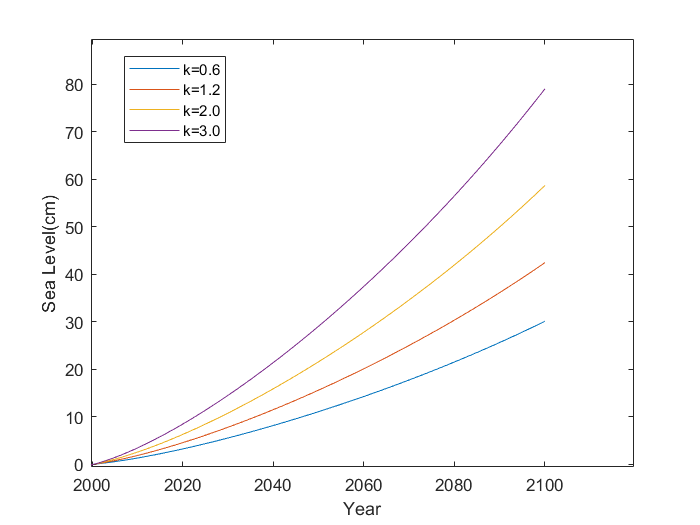
\includegraphics[width=.6\textwidth]{2000_2100.png}
	\caption{ The  estimated  global sea-level rise trend}\label{2000_2100}
\end{figure}


% Table generated by Excel2LaTeX from sheet 'Sheet2'
\begin{table}[htbp]
  \centering
  \caption{Sea level forecast for a particular year}
    \begin{tabular}{c|ccc}
    \toprule
    \multicolumn{1}{l|}{\kappa} & 2030  & 2050  & 2100 \\
    \midrule
    0.6   & 5.5   & 11.1  & 30.1 \\
    1.2   & 7.8   & 15.6  & 42.4 \\
    2     & 10.8  & 21.6  & 58.6 \\
    3     & 14.5  & 29    & 78.9 \\
    \bottomrule
    \end{tabular}%
  \label{Sea level forecast for a particular year}%
\end{table}%





The difference between the model and the real data(data source: NASA) is shown in Figure \ref{2000_2010}. We use mean square error (MSE) to compare the differences between the 4 models and the real data. The MSE values of the four models are 4.78, 2.29, 0.43, 0.38 respectively. When $\kappa = 3$, the model fits best.

\begin{figure}[htbp]
	\centering
	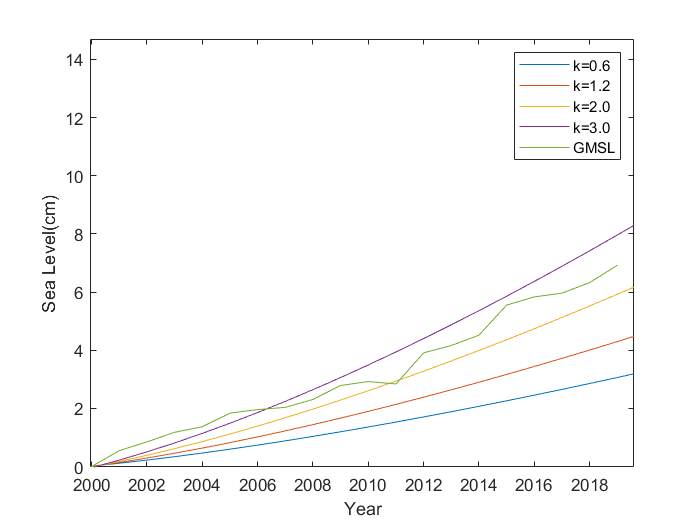
\includegraphics[width=.6\textwidth]{2000_2010.png}
	\caption{ The difference between the model and the real data}\label{2000_2010}
\end{figure}






%5.2
\subsection{The Risky Area and Population}

It can be seen from the above prediction that sea level will rise by 78.9cm in 2100 relative to 2000. This rise will result in the inundation and salinization of large areas of land in many coastal areas and islands. Then the land becomes uninhabitable, and the people who lived on it must move to other lands. For coastal countries with large landmasses, their at-risk populations will naturally migrate within their borders without creating environmental refugees. 

By contrast, island nations have no more room to accommodate their citizens who have lost their homes because of rising seas, so we can consider they are potential environmental refugees.
 For different types of island nations, however, the effects of rising sea levels on land flooding and salinization are different. Over this century, large swathes of island countries (such as Japan and Britain) will have plenty of land to house their at-risk populations. On the contrary, for small island countries, because the whole country is in the risk zone, there are a large number of potential environmental refugees.
 
Across the globe, we have picked out island countries smaller than 30,000km$^2$ and identified their inhabitants as potential environmental refugees. 
A total of 37 island states are threatened (see appendix for details) with a current population of 30,460,103. The geographical location is shown below.


\begin{figure}[htbp]\label{5.2}
	\centering
	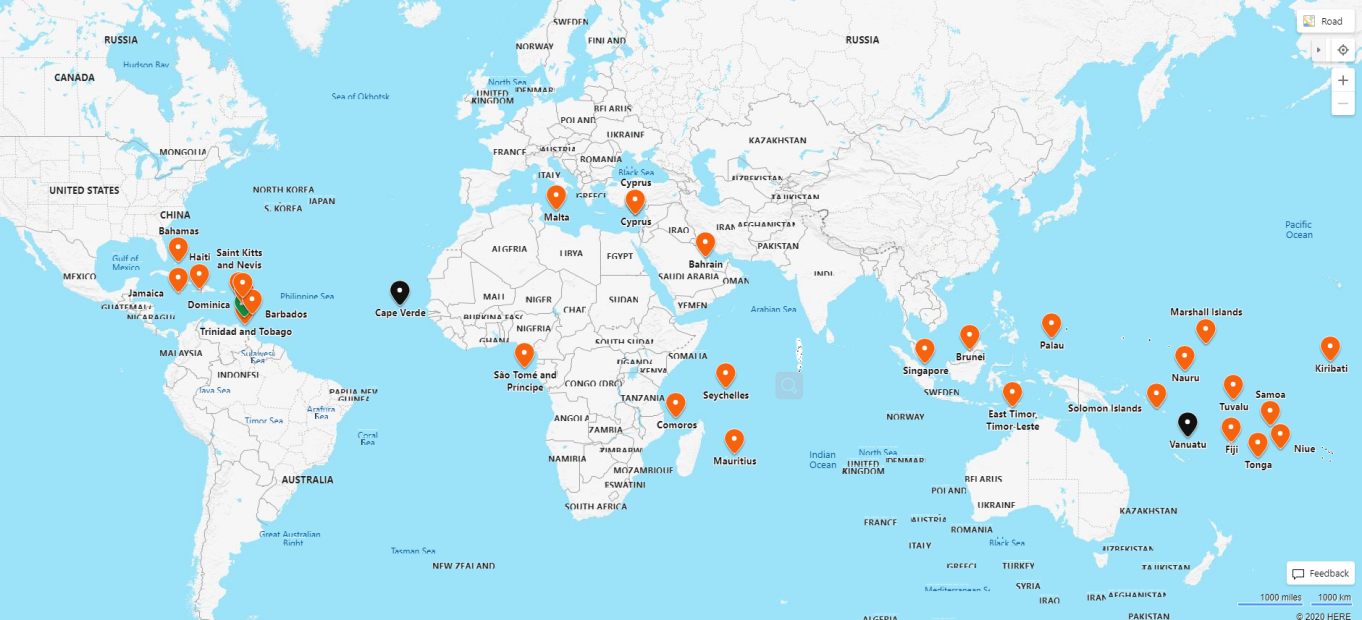
\includegraphics[width=1\textwidth]{5.2.png}
	\caption{ flow diagram of solution}\label{5.2}
\end{figure}




%6
\section{Preservation of Culture Policy}

%6.1
\subsection{The risk of loss of culture}


%6.2
\subsection{Concrete Policies}



%6.2.1
\subsubsection{Local Language}
Language can reflect the world outlook, the way of thinking, social characteristics, and culture of the user's nation. The main reason for the demise of languages is that society is moving towards more politically and economically dominant languages. Generally speaking, the language of the host country is more influential than the minor languages of the EDPs country, so it is necessary to protect the minor languages used by EDPs after they migrate to host countries.

%6.2.2
\subsubsection{Intangible Cultural Heritage}

(1)\textbf{Promote the intangible cultural heritage of at-risk island countries.}Through the media and other means to actively spread and increase external publicity, this can not only increase the residents' understanding of the culture of the EDPs but also reduce the cultural conflicts between residents and EDPs in the host countries. At the same time, museums should be set up actively, which can not only protect the tangible cultural heritage but also transform the intangible cultural heritage into videos, pictures, and other media.


(2)\textbf{The host country should make laws and regulations to protect EDPs.} A large number of refugees from the host country may lead to cultural conflicts such as customs and languages between the EDPs and the original residents. The host country should make similar laws and regulations to protect the culture of refugees and avoid discrimination against EDPs by residents.







%6.2.3
\subsubsection{Tangible Cultural Heritage}

(1)\textbf{Build museums to preserve the unique cultural relics.} The governments of EDPs countries should actively excavate and preserve local cultural relics and, in cooperation with the host countries, establish museums in the host countries in advance to display and protect their unique historical relics.



(2)\textbf{Establish an expert group to design plans for the removal of cultural sites.} Many of the cultural heritage sites of at-risk island nations are under threat, with many of them likely to be submerged as sea levels rise. Cultural sites should be relocated as soon as possible, or we have to prepare for marine protection. 



%7
\section{The Model for EDPs’ Migration}

%7.1
\subsection{}



%7.2
\subsection{}




%7.3
\subsection{}





%7.4
\subsection{}




%8
\section{Policies for Protection of Human Rights}


%%%%%%%%%%%%%%%%%%%%%%%%%%%%%%%%%%%%%%%%%%%%%%%%%%%%%%%%%%%%%%%%%%%%

% 参考文献,此处以 MLA 引用格式为例
\begin{thebibliography}{99}
\bibitem{1} Einstein, A., Podolsky, B., \& Rosen, N. (1935). Can quantum-mechanical description of physical reality be considered complete?. \emph{Physical review}, 47(10), 777.
\bibitem{2} \emph{A simple, easy \LaTeX\ template for MCM/ICM: EasyMCM}. (2018). Retrieved December 1, 2019, from\url{https://www.cnblogs.com/xjtu-blacksmith/p/easymcm.html}
\end{thebibliography}
%%%%%%%%%%%%%%%%%%%%%%%%%%%%%%%%%%%%%%%%%%%%%%%%%%%%%%%%%%%%%%%%%%%%%





% 如您的论文中不需要附录,请自行删除
\begin{subappendices}  % 附录环境

\section{Appendix A: Further on \LaTeX}
To clarify the importance of using \LaTeX\ in MCM or ICM, several points need to be covered, which are \ldots

To be more specific, \ldots

All in all, \ldots

Anyway, nobody \textbf{really} needs such appendix \ldots

\end{subappendices}



%%%%%%%%%%%%%%%%%%%%%%%%%%%%%%%%%%%%%%%%%%%%%%%%%%%%%%%%%%%%%%%%%%%%%%%%%


\section{XXXXXXXXXXXXXXXXXXXXXXXXXXXXXXXXXXXXXX}

Above all, in terms of the number of containers, it is obvious that more containers can provide more drones and medical supply. 

In addition, the area where the phrasecontainer is located can charge the drones. 
	
	Therefore, more containers will makethe drones more flexible and create a wider reconnaissance range. The most important point is that one or two cargo containers cannot cover the five hospitals(this will be shown in Part 7). Due to the reasons above, we firstly consider the
	number of containers is 3.
	
	We think the helicopter has the ability to transport containers to inland. Therefore, in terms of the location of the container, we need to consider the location of the container inside Puerto Rico so that the container can meet the daily needs of
	the hospital and the road reconnaissance.


\begin{table}[htbp]
	\centering
	\caption{Sea level prediction at a specific time}
	\begin{tabular}{c|ccc}
		\toprule
		\kappa     & 2030  & 2050  & 2100 \\
		\midrule
		0.634 & 9.45  & 15.48 & 32.28 \\
		1.2   & 10.89 & 17.82 & 37.16 \\
		2     & 12.19 & 19.95 & 41.6 \\
		3     & 13.3  & 21.83 & 45.5 \\
		\bottomrule
	\end{tabular}%
	\label{tab:addlabel}%
\end{table}%





%The detail can be described by equation \eqref{eq:heat}:
%\begin{equation}\label{eq:heat}
%\frac{\partial u}{\partial t} - a^2 \left( \frac{\partial^2 u}{\partial x^2} + \frac{\partial^2 u}{\partial y^2} + \frac{\partial^2 u}{\partial z^2} \right) = f(x, y, z, t)
%\end{equation}
\begin{figure}[htbp]
	\centering
	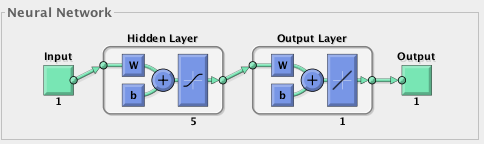
\includegraphics[width=.6\textwidth]{p1.png}
	\caption{ flow diagram of solution}\label{fig: flow diagram of solution}
\end{figure}



\subsection{Model 2}
The results are shown in Figure \ref{fig: flow diagram of solution}, where $t$ denotes the time in seconds, and $c$ refers to the concentration of water in the boiler.

\begin{figure}[htbp]
\centering
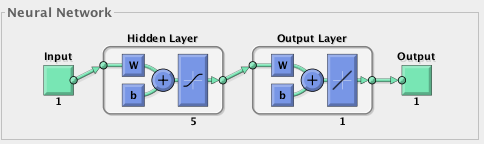
\includegraphics[width=.6\textwidth]{p1.png}
\caption{ flow diagram of solution}\label{fig: flow diagram of solution}
\end{figure}
We get the following equation\eqref{eq:complex}
\begin{equation}\label{eq:complex}
		T=\frac{D\times    V_m}{\sum_{i=1}^{n_d}{\frac{z_i}{\frac{d_i}{v_i+T_0}}}}
\end{equation}
\newpage
\section{Strengths and Weaknesses}
\subsection{Strengths}
\begin{itemize}
    \item First one...
    \item Second one ...
\end{itemize}
\begin{figure}[htbp]
	\begin{minipage}{0.45\linewidth}
		\centering
		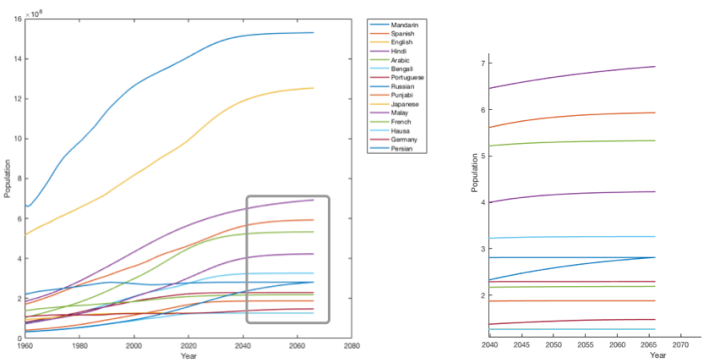
\includegraphics[width=\textwidth]{p3.png}
		\caption{Geometrical relationship} 
		\label{fig:beta}
	\end{minipage}
	\begin{minipage}{0.45\linewidth}
		\centering
		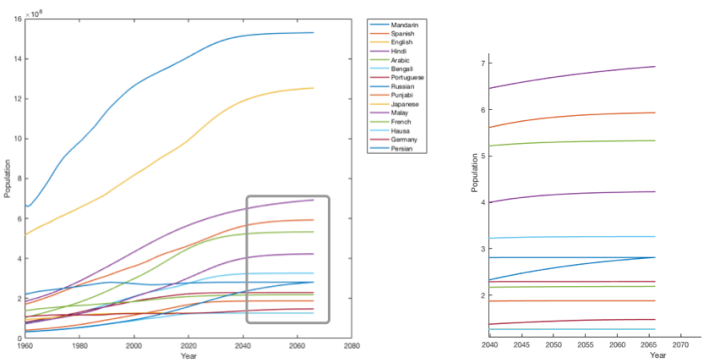
\includegraphics[width=\textwidth]{p3.png}
		\caption{The $F_s$ under ND control}
		\label{fig:Force_plane}
	\end{minipage}
\end{figure} 

\subsection{Weaknesses}
\begin{itemize}
    \item Only one ...
 \end{itemize}


% 以下为信件/备忘录部分,不需要可自行去掉
% 如有需要可将整个 letter 环境移动到文章开头或中间
% 请在后一个花括号内填写信件(Letter)或备忘录(Memorandum)标题
\begin{letter}{Memorandum}
\begin{flushleft}  % 左对齐环境,无首行缩进
\textbf{To:} Heishan Yan\\
\textbf{From:} Team XXXXXXX\\
\textbf{Date:} October 1st, 2019\\
\textbf{Subject:} A better choice than MS Word: \LaTeX
\end{flushleft}

In the memo, we want to introduce you an alternate typesetting program to the prevailing MS Word: \textbf{\LaTeX}. In fact, the history of \LaTeX\ is even longer than that of MS Word. In 1970s, the famous computer scientist Donald Knuth first came out with a typesetting program, which named \TeX\ \ldots

Firstly, \ldots

Secondly, \ldots

Lastly, \ldots

According to all those mentioned above, it is really worth to have a try on \LaTeX! 
\end{letter}


% 参考文献,此处以 MLA 引用格式为例
\begin{thebibliography}{99}
\bibitem{1} Einstein, A., Podolsky, B., \& Rosen, N. (1935). Can quantum-mechanical description of physical reality be considered complete?. \emph{Physical review}, 47(10), 777.
\bibitem{2} \emph{A simple, easy \LaTeX\ template for MCM/ICM: EasyMCM}. (2018). Retrieved December 1, 2019, from\url{https://www.cnblogs.com/xjtu-blacksmith/p/easymcm.html}
\end{thebibliography}


% 以下为附录内容

\end{document}